%%%%%%%%%%%%%%%%%%%%%%%%%%%%%%%%%%%%%%%%%
% Short Sectioned Assignment
% LaTeX Template
% Version 1.0 (5/5/12)
%
% This template has been downloaded from:
% http://www.LaTeXTemplates.com
%
% Original author:
% Frits Wenneker (http://www.howtotex.com)
%
% License:
% CC BY-NC-SA 3.0 (http://creativecommons.org/licenses/by-nc-sa/3.0/)
%
%%%%%%%%%%%%%%%%%%%%%%%%%%%%%%%%%%%%%%%%%

%----------------------------------------------------------------------------------------
%	PACKAGES AND OTHER DOCUMENT CONFIGURATIONS
%----------------------------------------------------------------------------------------

\documentclass[paper=a4, fontsize=11pt]{scrartcl} % A4 paper and 11pt font size

\usepackage[T1]{fontenc} % Use 8-bit encoding that has 256 glyphs
\usepackage{fourier} % Use the Adobe Utopia font for the document - comment this line to return to the LaTeX default
\usepackage[spanish]{babel} % English language/hyphenation
\selectlanguage{spanish}
\usepackage[utf8]{inputenc}
\usepackage{amsmath,amsfonts,amsthm} % Math packages
\usepackage{graphicx}

\usepackage{sectsty} % Allows customizing section commands
\allsectionsfont{\centering \normalfont\scshape} % Make all sections centered, the default font and small caps

\usepackage{fancyhdr} % Custom headers and footers
\pagestyle{fancyplain} % Makes all pages in the document conform to the custom headers and footers
\date{}
\fancyhead{} % No page header - if you want one, create it in the same way as the footers below
\fancyfoot[L]{} % Empty left footer
\fancyfoot[C]{} % Empty center footer
\fancyfoot[R]{\thepage} % Page numbering for right footer
\renewcommand{\headrulewidth}{0pt} % Remove header underlines
\renewcommand{\footrulewidth}{0pt} % Remove footer underlines
\setlength{\headheight}{9.6pt} % Customize the height of the header

\numberwithin{equation}{section} % Number equations within sections (i.e. 1.1, 1.2, 2.1, 2.2 instead of 1, 2, 3, 4)
\numberwithin{figure}{section} % Number figures within sections (i.e. 1.1, 1.2, 2.1, 2.2 instead of 1, 2, 3, 4)
\numberwithin{table}{section} % Number tables within sections (i.e. 1.1, 1.2, 2.1, 2.2 instead of 1, 2, 3, 4)

\setlength\parindent{0pt} % Removes all indentation from paragraphs - comment this line for an assignment with lots of text

%----------------------------------------------------------------------------------------
%	TITLE SECTION
%----------------------------------------------------------------------------------------

\newcommand{\horrule}[1]{\rule{\linewidth}{#1}} % Create horizontal rule command with 1 argument of height

\title{	
\normalfont \normalsize 
\textsc{UNIVERSIDAD DE CANTABRIA, DEPARTAMENTO DE FÍSICA MODERNA} \\ [20pt] % Your university, school and/or department name(s)
\horrule{0.5pt} \\[0.4cm] % Thin top horizontal rule
\huge Física de Partículas Elementales (G71) \\ % The assignment title
\normalsize 4 Curso - Grado de Física (31 de Enero de 2018)
\horrule{2pt} \\[0.5cm] % Thick bottom horizontal rule
}

\begin{document}

\maketitle % Print the title

\vspace{-2.5cm}

%----------------------------------------------------------------------------------------
%	PROBLEM 1
%----------------------------------------------------------------------------------------
\textbf{Cuestión 1.} Demuestra que el proceso $\gamma \rightarrow e^{+}e^{-}$ no puede producirse en el vacío (1 punto). Encuentra el máximo ángulo de apertura entre los fotones producidos en el decaimiento
$\pi^{0}\rightarrow\gamma\gamma$ si la energía total del pion es 10 GeV, teniendo en cuenta que la masa del pion es 135 MeV (1 punto). 
\\
\\
%----------------------------------------------------------------------------------------
%	PROBLEM 2
%----------------------------------------------------------------------------------------
\textbf{Cuestión 2.} Utilizando la expresión $(\gamma^\mu p_\mu - m)u = 0$ obten la expresión para el spinor adjunto $\bar{u}(\gamma^\mu p_\mu - m) = 0$ sabiendo que $\{\gamma^\mu, \gamma^\nu\}=2g^{\mu\nu}$ (1 punto). 
Sin utilizar las expresiones explíticas para los espinores $u$, muestra que si tenemos la condición de normalización $u^\dag u=2E$, entonces $\bar{u}u = 2m$ (1 punto). \textbf{Pista:} Multiplica $\bar{u}\gamma^\nu$ por la
izquierda a $(\gamma^\mu p_\mu - m)u = 0$ y $\gamma^\nu u$ por la derecha a $\bar{u}(\gamma^\mu p_\mu - m) = 0$, súmalas y considera el caso $\nu=0$ sabiendo que $(\gamma^0)^2=1$.
%----------------------------------------------------------------------------------------
\\
\\
%----------------------------------------------------------------------------------------
%       PROBLEM 3
%----------------------------------------------------------------------------------------
\textbf{Cuestión 3.} Escribir la expresión de la regla de oro de Fermi y discutir el significado de los diferentes términos (1 punto). Considera el proceso weak $e^{-}\nu_\mu\rightarrow\nu_e\mu^{-}$: dibuja
el diagrama de Feynman asociado de primer orden (0.5 puntos). Con ayuda de las reglas de Feynmann indica la estructura que tendría el elemento de matriz asociado, explicando brevemente lo que es cada término (0.5 puntos).  
%----------------------------------------------------------------------------------------
\\
\\
%----------------------------------------------------------------------------------------
%       PROBLEM 4
%----------------------------------------------------------------------------------------
\textbf{Cuestión 4.} Definir el concepto de helicidad y de quiralidad (0.5 puntos). Explica la relación que existe entre el hecho de que la fuerza débil viola la simetría CP y que los bosones W solo interaccionen
con la parte left-handed de las partículas (right-handed para antipartículas) (1 punto). Demostrar las siguientes relaciones entre los operadores de proyección quiral (chiral): $P_{R} + P_{L} = 1$, $P_{R} P_{R} = P_{R}$, $P_{L} P_{L} = P_{L}$ y $P_R P_L = 0$.
\textbf{Pista:} Recuerda que $(\gamma^5)^2=1$ en donde

\begin{equation*}
\gamma^5 = i\gamma^0\gamma^1\gamma^2\gamma^3 = 
\begin{bmatrix}
    0 & I_{2x2} \\
    I_{2x2} & 0 
\end{bmatrix} 
\end{equation*}
\\
\\
\textbf{Cuestión 5.} El $\pi^{-}$ se desintegra vía interacción débil cargada en un par de leptones. Experimentalmente se encuentra que:

\begin{equation*}
\frac{\Gamma\left (\pi^{-}\rightarrow e^{-}\bar{\nu_e}\right )}{\Gamma\left (\pi^{-}\rightarrow \mu^{-}\bar{\nu_\mu}\right )} = 1.23\times 10^{-4}
\end{equation*}
Discutir el papel de la helicidad para que se verifique esta relación.

\begin{figure}
\begin{center}
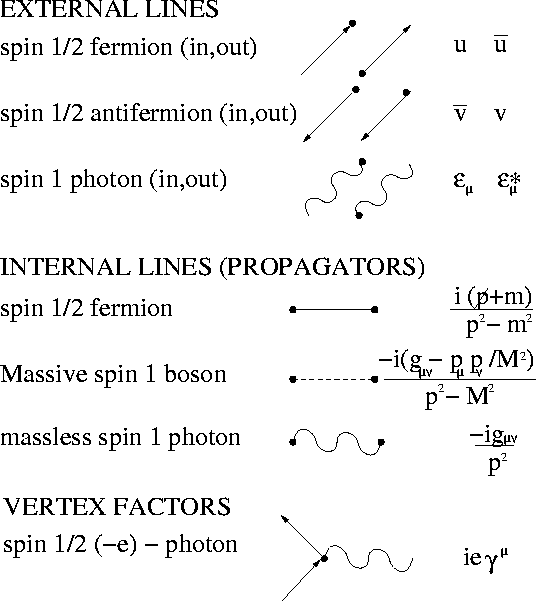
\includegraphics[width=0.5\linewidth]{feynmanrules.png}
\end{center}
\end{figure}

\end{document}
